% ===================================================================================================================
% Section III body (paste under \section{Spatiotemporal Packing} \label{sec:packing}).
% Needs in the preamble:  \usepackage[ruled,vlined,linesnumbered]{algorithm2e}
% Alg. 1 = pack_weights() and Alg. 2 = pack_spikes() of ours.py, line for line (the RTL-verified cycle model).
% Example values = Fig. 3(d) / DAC2027_accelerator_explained_rows.pdf (second filter: weight 1 on K2). The figure's
% groups {P0,P1},{P2,P3} are Alg. 2 with G_max = 2; with G_max = 4 it gives {P0,P1,P3},{P2} (still 8 passes).
% ===================================================================================================================
DPTP packs both operands before they enter the array, so no packing decision is made inside it. \emph{Filter
packing} merges filters into array columns; it is computed offline, and the packed weights are stored with their
labels. Spike trains exist only at run time, so TIP merges output positions into packed trains in a pre-processing
unit at the edge of the array, just before they are fed in (Section~\ref{sec:arch}). Both work on one tile
$\mathcal{K}$ of $R$ inputs and are redone for every tile.

\subsection{Basic Concept}
\label{sec:pack-concept}
In Eq.~\eqref{eq:gemm}, the input index $k$ is the dimension shared by the spike trains and the weights. The other
two dimensions, output positions $m$ and filters $n$, can be merged without changing the result. The difference is the entry being merged: an entry of the spiking GEMM is a $T$-bit
spike train, so two output positions can share a packed train whenever they satisfy Eq.~\eqref{eq:tip}, not only
when they satisfy Eq.~\eqref{eq:atomic}.

In Fig.~\ref{fig:modes}(d), with $G_{\max} = 2$, P0 and P1 fire at different timesteps on K2 and are never both
non-silent on another input, so they form one group. P2 conflicts with P1 on K1 at $t_2$ and starts a second
group, which P3 joins. The two filters have non-zeros at disjoint inputs, so filter packing places both on one
column. Four packed trains per group and one weight column give 8 PE-passes for the whole GEMM.

\subsection{Label Format and Dataflow}
\label{sec:pack-format}
Labels name only the merged dimensions. Each weight carries a $\lceil \log_2 F_{\max} \rceil$-bit filter label,
and each spike of a packed train carries a $\lceil \log_2 G_{\max} \rceil$-bit label $\ell_{G,k}[t]$ naming its
member; the timestep needs no label, because it is the spike's place in the train.

The packed trains $\hat{\mathbf{s}}_{G,k}$ of a group stream along the rows of the tile, and the group carries
$F_{\max} G_{\max}$ partial sums down each column, one per (filter, member). In one cycle, a PE adds its weight to
every timestep at which the packed train fires, and the filter label and $\ell_{G,k}[t]$ select the partial sum.
In the example, the PE in row K2 holds the weight 1 of the second filter and receives the packed train 0111 of
the first group with labels (--, P0, P1, P1): it adds 1 to the partial sum of P0 at $t_1$ and to that of P1 at
$t_2$ and $t_3$. A PE holds at most one non-zero weight and a packed train at most one spike per timestep, so
every addition has exactly one destination. An output buffer sums the tiles.

\subsection{Packing Algorithms}
\label{sec:pack-alg}
Both packings are bounded graph coloring: output positions (or filters) are vertices, joined
by an edge when they conflict, and a group (or column) is an independent set of at most $G_{\max}$ (or $F_{\max}$)
vertices. We solve both greedily by first-fit on bit masks: filter packing offline, and TIP in the pre-processing
unit.

In Algorithm~\ref{alg:filter}, the mask of a filter marks the inputs of $\mathcal{K}$ where its weight is non-zero
(line 2). Filters without a non-zero weight in the tile are dropped, and the rest are taken densest first
(line 3). Each joins the first column with fewer than $F_{\max}$ filters and no overlapping input (lines 5--8), or
opens a new column (line 9).

In Algorithm~\ref{alg:tip}, the mask of an output position holds its $R \times T$ spikes on $\mathcal{K}$, so the
AND of two masks is zero exactly when the pair satisfies Eq.~\eqref{eq:tip}. Positions silent on the whole tile are
skipped (line 3). A position joins the oldest open group it does not overlap (lines 5--7), and a group with
$G_{\max}$ members is closed (line 8). Otherwise the position opens a group, and if $Q$ groups are already open,
the oldest is closed first (lines 10--12). The open groups are closed at the end of the tile (line 13).

\begin{algorithm}[t]
  \caption{Filter Packing}
  \label{alg:filter}
  \small
  \SetKwProg{Fn}{Function:}{}{}
  \KwIn{$w_{k,n}$ for $k \in \mathcal{K}$; threshold $F_{\max}$}
  \KwOut{$cols$, the filters packed into each array column}
  \Fn{}{
    \lFor{$n$ \textbf{in} filters}{$mask_n = (w_{k,n} \neq 0)_{k \in \mathcal{K}}$}
    $order = sort\_by\_nnz(\{n : mask_n \neq 0\})$\;
    \For{$n$ \textbf{in} $order$}{
      \For{$c$ \textbf{in} $cols$}{
        \If{$c.size() < F_{\max}$ \textbf{and} $(c.mask\ \&\ mask_n) == 0$}{
          $c.merge(n,\ mask_n)$\;
          \textbf{break}\;
        }
      }
      \lIf{$n$ not merged}{$cols.push(n,\ mask_n)$}
    }
    \Return $cols$\;
  }
\end{algorithm}

\begin{algorithm}[t]
  \caption{Timestep-Interleaved Packing}
  \label{alg:tip}
  \small
  \SetKwProg{Fn}{Function:}{}{}
  \KwIn{$mask_m = (s_{m,k}[t])_{k \in \mathcal{K},\, t < T}$ for the output positions $m$; threshold $G_{\max}$;
        open groups $Q$}
  \KwOut{$groups$, the groups $G$ of tile $\mathcal{K}$}
  \Fn{}{
    \For{$m$ \textbf{in} positions}{
      \lIf{$mask_m == 0$}{\textbf{continue}}
      $mergedFlag = 0$\;
      \For{$G$ \textbf{in} $open$}{
        \If{$(G.mask\ \&\ mask_m) == 0$}{
          $G.merge(m,\ mask_m)$;\ \ $mergedFlag = 1$\;
          \lIf{$G.size() == G_{\max}$}{$groups.push(open.pop(G))$}
          \textbf{break}\;
        }
      }
      \If{$mergedFlag == 0$}{
        \lIf{$open.size() == Q$}{$groups.push(open.pop\_oldest())$}
        $open.push(m,\ mask_m)$\;
      }
    }
    $groups.push(open)$\;
    \Return $groups$\;
  }
\end{algorithm}

\begin{figure*}[t]
  \centering
  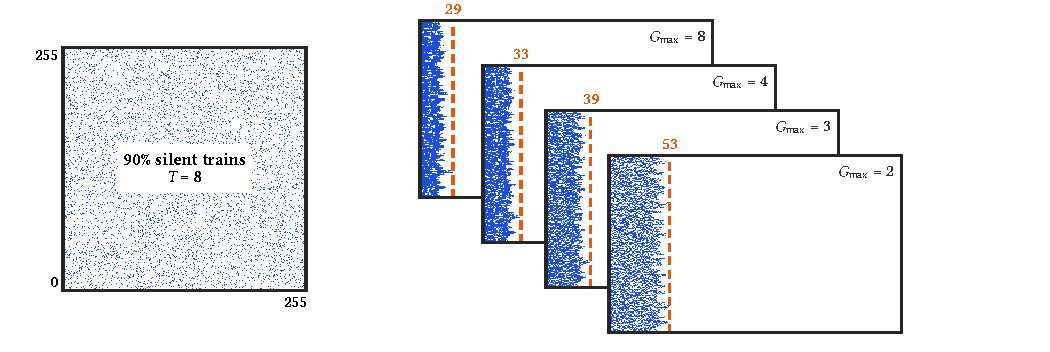
\includegraphics[width=\textwidth]{Figures/tip_visual.pdf}
  \caption{TIP at different thresholds $G_{\max}$. Left: a $256 \times 256$ spike matrix with 90\% silent trains and
  $T = 8$. Right: the packed matrix for each $G_{\max}$, built per tile of four inputs and 128 output positions;
  each column is one group, and the dashed line marks the widest tile.}
  \label{fig:thresholds}
\end{figure*}

\subsection{Thresholds}
\label{sec:pack-thresholds}
Two thresholds bound the packing: $G_{\max}$ limits the members of a group and $F_{\max}$ the filters of
a column. Larger thresholds merge more but widen the labels and the $F_{\max} G_{\max}$ partial sums each column
carries (Fig.~\ref{fig:thresholds}). $Q$ bounds the open groups each position is tested against. TIDES uses
$G_{\max} = F_{\max} = Q = 4$, giving 2-bit labels and 16 partial sums per column.
